\chapter{Mengenal Python dan Anaconda}

\section{Teori}
\subsection{Sejarah Python}
Nama python berasal dari acara televisi Monty python's flying circus. Python merupakan bahasa pemrograman yang dikembangkan oleh Guido Van Rossum pada tahun 1990 di CWI, Amsterdam. bahasa ini merupakan lanjutan dari bahasa pemrograman ABC. pada tahun 1995, Guido pindah ke CNRI dan mengeluarkan python versi 1.6. pada tahun 2000, Guido pindah ke BeOpen dan mengeluarkan python versi 2.0 setelah itu Guido dan tim PythonLabs pindah ke  DigitalCreations. saat ini Guido dan Python Software Foundation terus melakukan perkembangan hingga python versi 2.6.1 dan python versi 3.0
Python Software Foundation merupakan sebuah organisasi yang memiliki hak atas bahasa pemrograman python, hal ini dilakukan untuk mencegah bahasa pemrograman python dimiliki oleh perusahaan komersial.
\subsection{Perbedaan Python 2 dan 3}
Perbedaan Python 2 dan Python 3 dapat dilihat pada gambar berikut.
\begin{figure}[H]
        \centerline{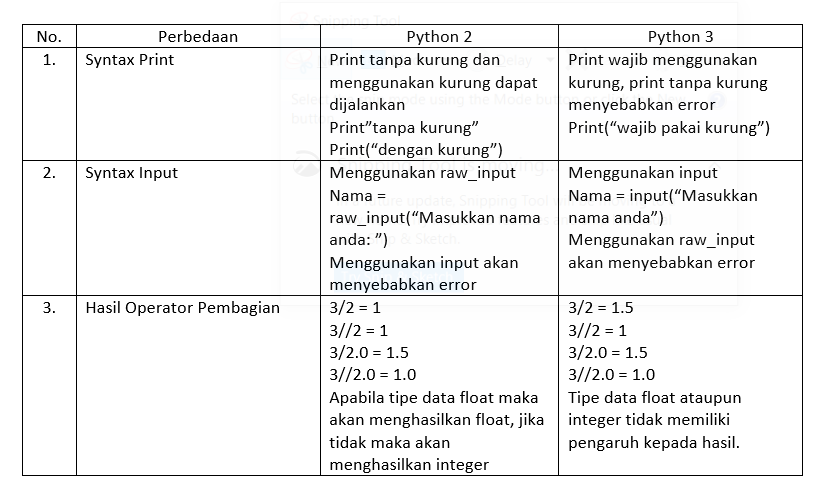
\includegraphics[scale=1]{figures/perbedaan}}
        \caption{Perbedaan Python 2 dan Python 3}
		\label{perbedaan}
\end{figure}

\subsection{Implementasi dan Penggunaan Python di Perusahaan Dunia}
\begin{enumerate}
\item spotify 
\par
spotify adalah suatu layanan musik streaming yang menggunakan pemrograman python untuk analisis data dan backend. pada backend spotify berkomunikasi dengan 0MQ. 0MQ itu sendiri  adalah suatu framework dan library open source untuk networking. untuk analisis data tersebut spotify menggunakan luigi, dan modul python yang sinkron dengan hadoop.
\item Google
\par 
Google ini sudah menggunakan bahasa pemprograman python ini sudah sajak dari awal berdirinya. Dan pada saat ini bahasa pemprograman python merupakan salah satu bahasa pemprograman server-side resmi di google. Meskipun ada script yang ditulis untuk google menggunakan bahasa perl dan bash, maka nantinya script tersebut akan diubah ke python terlebih dahulu, karena kemudahan dalam perawatannya.
\item Industrial Light and Magic
\par 
Industrial Light and Magic ini merupakan studio special efek yang dibutuhkan untuk film star wars saja. Karena infrastruktur awal industrial light and magisc ini menggunakan C dan C++, maka akan lebih mudah mengintegrasikan bahasa pemprograman python ketimbang bahasa pemprograman lainnya. Dengan menggunakan bahasa pemprogramana python ini industrial light and magic dengan mudah membungkus komponen software dan dapat meningkatkan aplikasi grafisnya.
\item Netflix
\par 
Netflix adalah suatu layanan pemutaran film yang dapat dilakukan oleh pengguna dimanapun dan kapanpun. Pada netfilx bahasa pemprograman yang digunakan adalah bahasa pemprograman python, bahasa pemprograman ini digunakan pada Central Alert Gateway yang akan me-reroute alert dan mengirimkannya pada individu yang akan melihatnya serta juga  dapat secara otomatis reboot atau menghentikan proses yang dianggap bermasalah. Selain itu python juga digunakan untuk menelusuri riwayat dan perubahan pengaturan keamanan.
\item instagram 
\par 
Instagram adalah suatu aplikasi mobile berbasis IOS, android dan windows phone, dimana pengguna dapat berbagi foto dan video melalui instagram ini. Pada instagram ini menggunakan bahasa pemprograman python dalam task queuennya atau fitur dimana setiap pengguna dapat berbagi foto atau video ke beberapa social network lainnya seperti facebook, twitter, dan lain-lainnya.

\end{enumerate}
\section{Instalasi}
\subsection{Instalasi Anaconda 3}
Hal yang harus diperhatikan sebelum melakukan instalasi \textit{Anaconda Python}
\begin{enumerate}
 \item Perhatikan versi dari sistem operasi yang digunakan (versi 32bit atau 64bit)
 \item Download file anaconda yang sesuai dengan versi sistem operasi (32bit atau 64bit)
 \item \textit{Download Anaconda Python} https://www.anaconda.com/distribution/
\end{enumerate}

Berikut langkah-langkah instalasi anaconda.
\begin{enumerate}
\item Buka aplikasi \textit{installer Anaconda} tersebut lalu akan muncul  gambar \textit{installer anaconda}.
\begin{figure}[H]
        \centerline{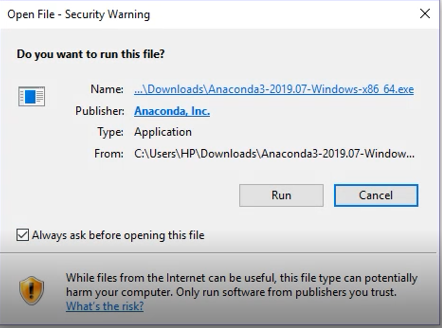
\includegraphics[scale=0.5]{figures/1}}
        \caption{Run Setup Anaconda}
		\label{langkah1}
\end{figure}

\item Tunggu hingga \textit{setup loading} selesai
\begin{figure}[H]
        \centerline{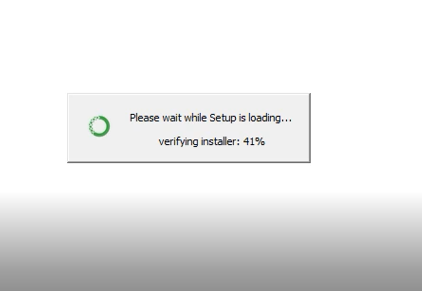
\includegraphics[scale=0.5]{figures/2}}
        \caption{Setup Loading}
		\label{langkah2}
\end{figure}


\item Jika \textit{setup loading} telah selesai, maka klik \textit{next}
\begin{figure}[H]
        \centerline{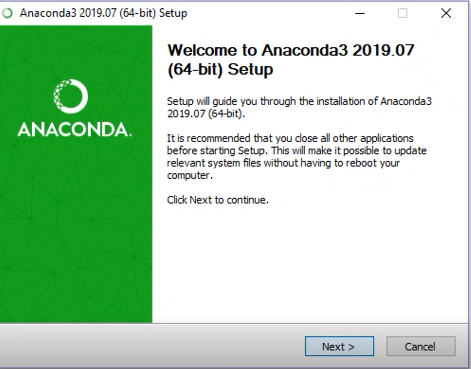
\includegraphics[scale=0.5]{figures/3}}
        \caption{Welcome to Anaconda Setup}
		\label{langkah2}
\end{figure}


\item Pada \textit{License Agreement} klik \textit{I Agree}
 gambar \textit{License Agreement}.

\begin{figure}[H]
    \centering
    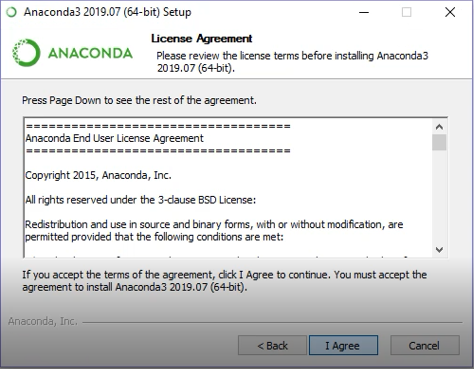
\includegraphics[scale=0.5]{figures/4}
    \caption{\textit{License Agreement}}
    \label{Figureanaconda3}
\end{figure}


\item Kemudian pilih \textit{Just Me(Recomended)} agar sesuai dengan komputer yang digunakan, kemudian klik \textit{next}
 gambar \textit{Just Me(recomended)}.

\begin{figure}[H]
    \centering
    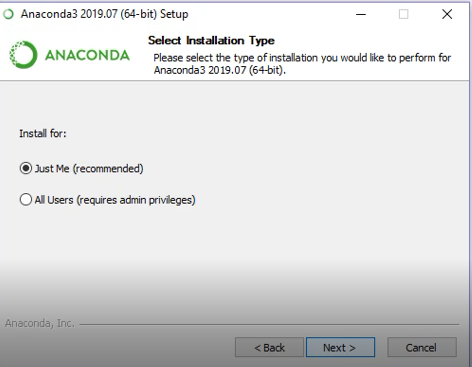
\includegraphics[scale=0.5]{figures/5}
    \caption{\textit{Just Me(recomended)}}
    \label{Figureanaconda4}
\end{figure}


\item Kemudian pilih lokasi tempat \textit{menginstall anaconda}
 gambar \textit{Pilih lokasi}.

\begin{figure}[H]
    \centering
    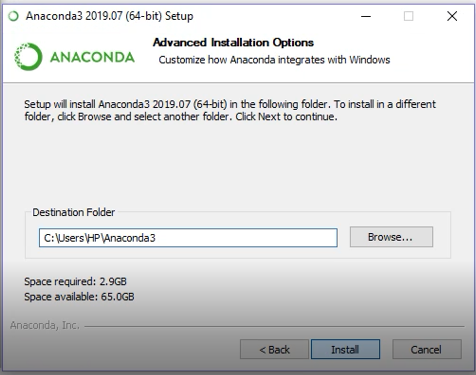
\includegraphics[scale=0.5]{figures/6}
    \caption{\textit{Pilih lokasi}}
    \label{Figureanaconda5}
\end{figure}

\item Kemudian centang \textit{Add Anaconda to my Path environtment variable}, agar saat \textit{menginstall selenium} langsung ke \textit{path anaconda} tidak ke aplikasi yang lain. Klik \textit{install}
 gambar \textit{Centang Anaconda to my PATH}.

\begin{figure}[H]
    \centering
    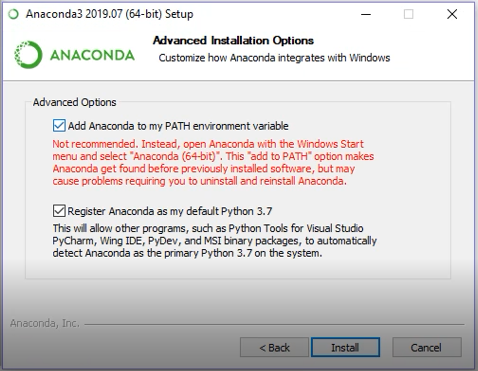
\includegraphics[scale=0.5]{figures/7}
    \caption{\textit{Centang Anaconda to my PATH}}
    \label{Figureanaconda6}
\end{figure}

\item Tunggu sampai proses \textit{installasi} selesai
 gambar \textit{Installation Complete}.

\begin{figure}[H]
    \centering
    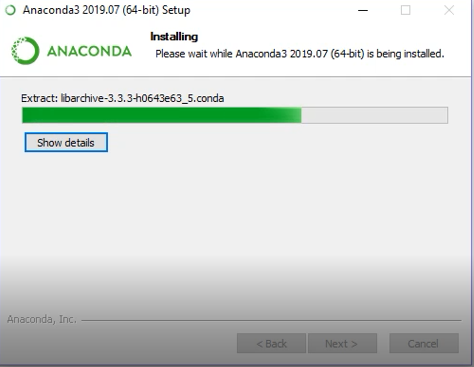
\includegraphics[scale=0.5]{figures/8}
    \caption{\textit{Installation Complete}}
    \label{Figureanaconda7}
\end{figure}

\item Apabila instalasi telah selesai klik \textit{next}
\begin{figure}[H]
    \centering
    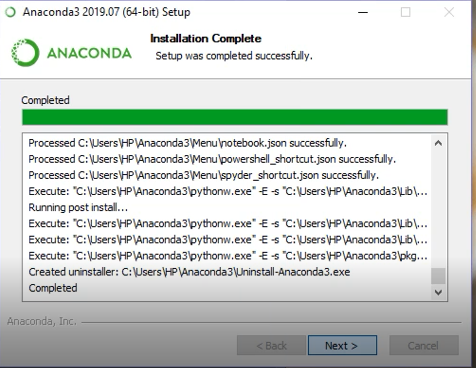
\includegraphics[scale=0.5]{figures/9}
    \caption{\textit{Installation Complete}}
    \label{Figureanaconda8}
\end{figure}

\item klik \textit{next}
\begin{figure}[H]
    \centering
    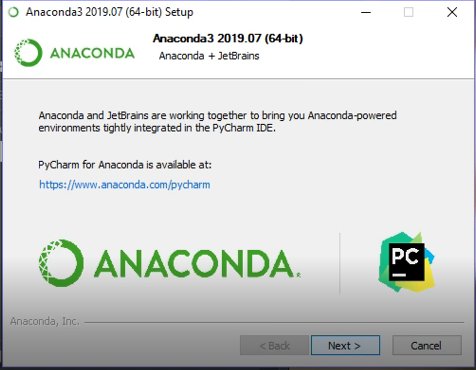
\includegraphics[scale=0.5]{figures/10}
    \caption{\textit{Anaconda+JetBrains}}
    \label{Figureanaconda70}
\end{figure}

\item Jika sudah klik \textit{finish}
 gambar \textit{Thanks fo install Anaconda}.

\begin{figure}[H]
    \centering
    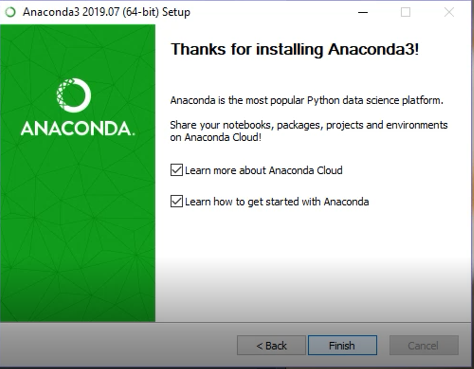
\includegraphics[scale=0.5]{figures/11}
    \caption{\textit{Thanks for install Anaconda}}
    \label{Figureanaconda70}
\end{figure}
\end{enumerate}

\subsection{Instalasi Pip}
\begin{enumerate}
\item buka anaconda promt
\item ketikkan conda install -c anaconda pip
\begin{figure}[H]
    \centering
    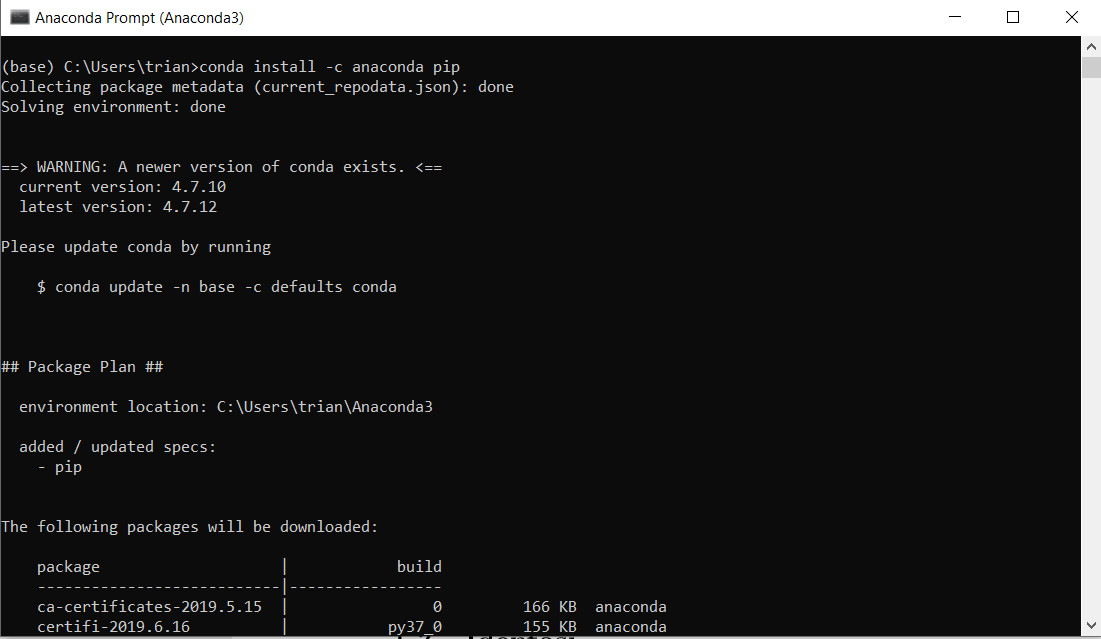
\includegraphics[scale=0.5]{figures/installpip}
    \caption{\textit{Install pip}}
    \label{Figureanaconda70}
\end{figure}
\item ketik y, lalu enter. Tunggu hingga proses instalasi selesai.
\begin{figure}[H]
    \centering
    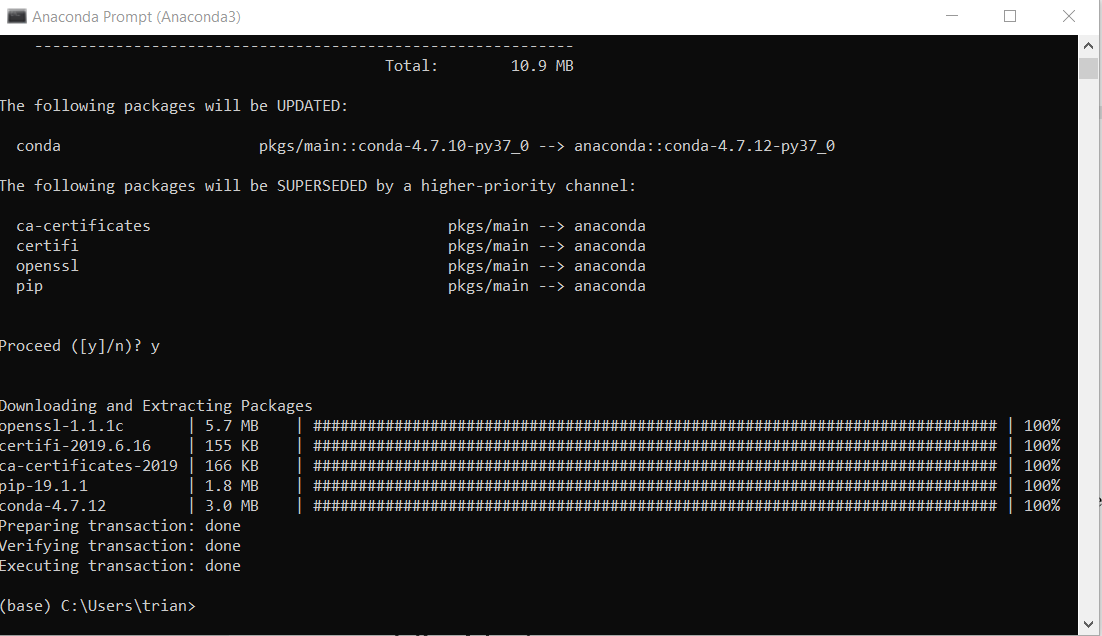
\includegraphics[scale=0.5]{figures/pipselesai}
    \caption{\textit{Install pip Selesai}}
    \label{Figureanaconda70}
\end{figure}
\item jika telah selesai, lakukan pengecekan versi pip dengan mengetikkan pip -V
\begin{figure}[H]
    \centering
    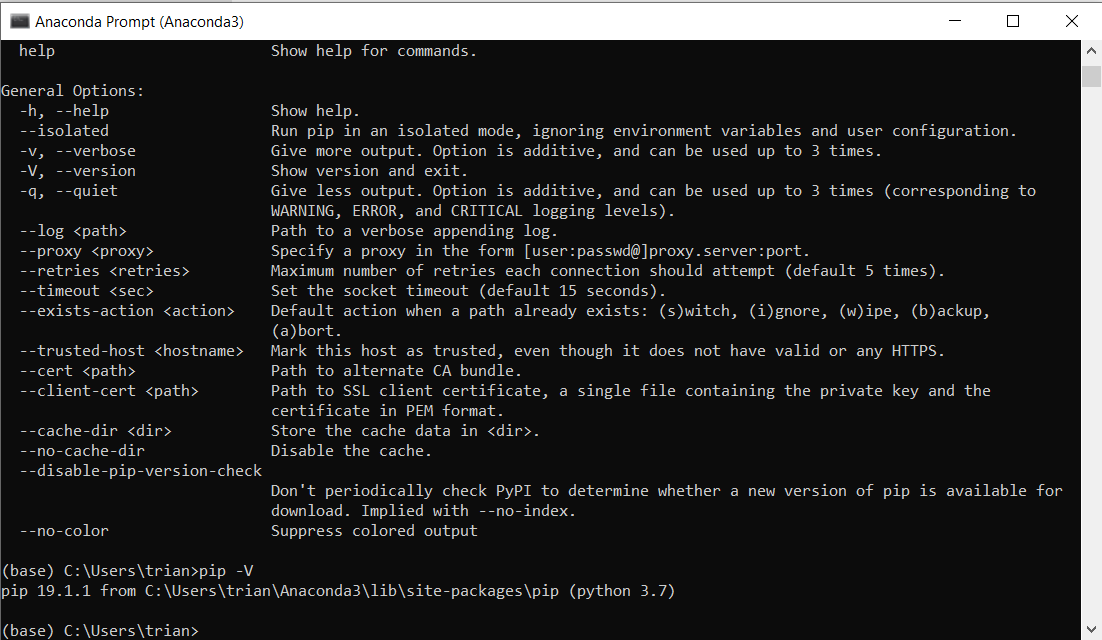
\includegraphics[scale=0.5]{figures/pipversion}
    \caption{\textit{Melihat Versi pip}}
    \label{Figureanaconda70}
\end{figure}

\end{enumerate}

\subsection{Setting Environment}
\begin{enumerate}
\item Buka file explorer
\item Klik kanan pada This pc, lalu pilih properties
\begin{figure}[H]
    \centering
    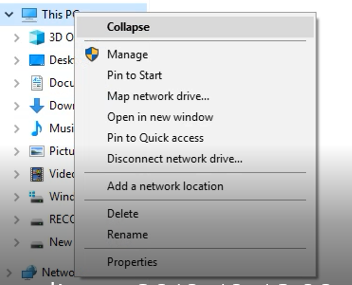
\includegraphics[scale=0.7]{figures/properties}
    \caption{\textit{Properties}}
    \label{Environment1}
\end{figure}
\item Pilih menu Advanced system settings
\begin{figure}[H]
    \centering
    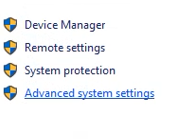
\includegraphics[scale=0.7]{figures/advanced}
    \caption{\textit{Advanced system settings}}
    \label{Environment2}
\end{figure}
\item Pilih Environment Variables
\begin{figure}[H]
    \centering
    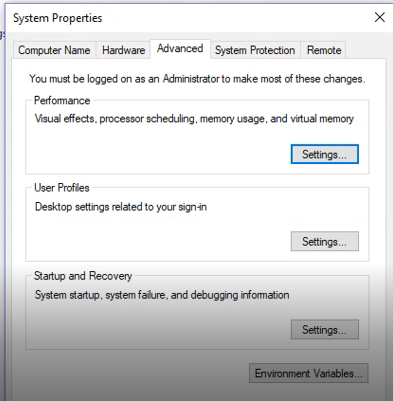
\includegraphics[scale=0.7]{figures/environment}
    \caption{\textit{Environment Variables}}
    \label{Environment3}
\end{figure}
\item Pilih Path
\begin{figure}[H]
    \centering
    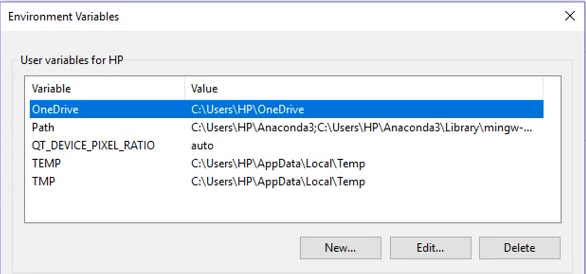
\includegraphics[scale=0.7]{figures/path}
    \caption{\textit{Path}}
    \label{Environment4}
\end{figure}
\item lalu pilih environment variable yang ingin ditambahkan, klik OK
\begin{figure}[H]
    \centering
    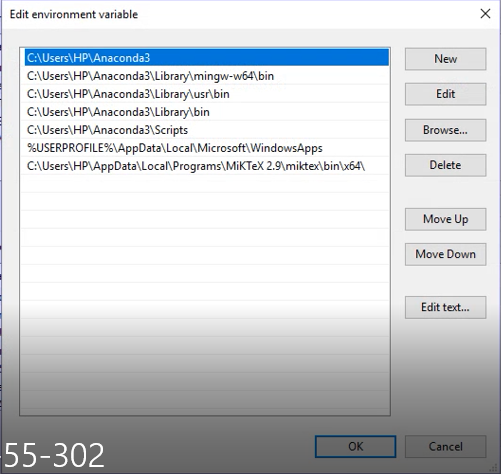
\includegraphics[scale=0.7]{figures/ok}
    \caption{\textit{Edit Environment Variable}}
    \label{Environment5}
\end{figure}
\end{enumerate}

\subsection{Command Line Interface/Interpreter}
\begin{enumerate}
\item Buka command prompt lalu ketikkan python
\item Buatlah perintah print, input, perkalian, dan pembagian
\item Bisa juga menjalankan file .py yang telah dibuat di IDE dengan cara python namafile.py, lalu klik enter
\begin{figure}[H]
    \centering
    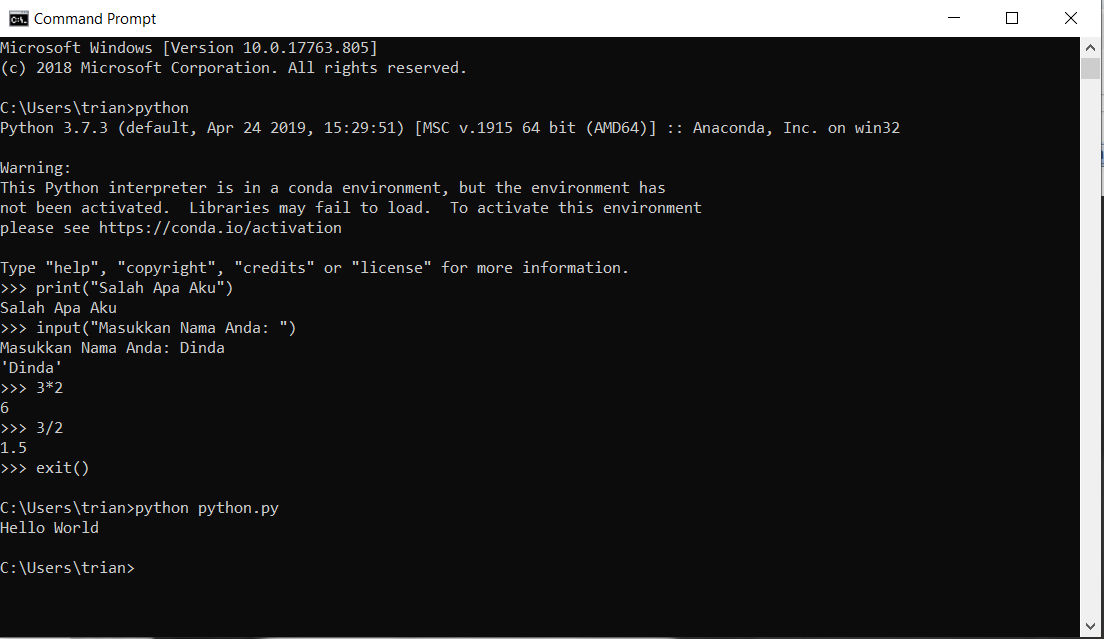
\includegraphics[scale=0.5]{figures/cli}
    \caption{\textit{CLI in Command Prompt}}
    \label{CLI}
\end{figure}
\end{enumerate}

\subsection{Update Anaconda dan Spyder}
Cara mengupdate Spyder
\begin{enumerate}
\item Buka anaconda prompt, lalu ketikkan perintah conda update spyder
\item Konfirmasi update dengan mengetikkan y, lalu tekan enter
\item Tunggu hingga installan selesai
\end{enumerate}
Cara mengupdate Anaconda
\begin{enumerate}
\item Buka anaconda prompt, lalu ketikkan perintah conda update anaconda
\item Konfirmasi update anaconda dengan mengetikkan y dan kemudian tekan enter
\item Tunggu hingga installan selesai
\end{enumerate}
\subsection{Run Script Hello World di Spyder}
\begin{enumerate}
\item Buka anaconda navigator, lalu klik launch
\begin{figure}[H]
    \centering
    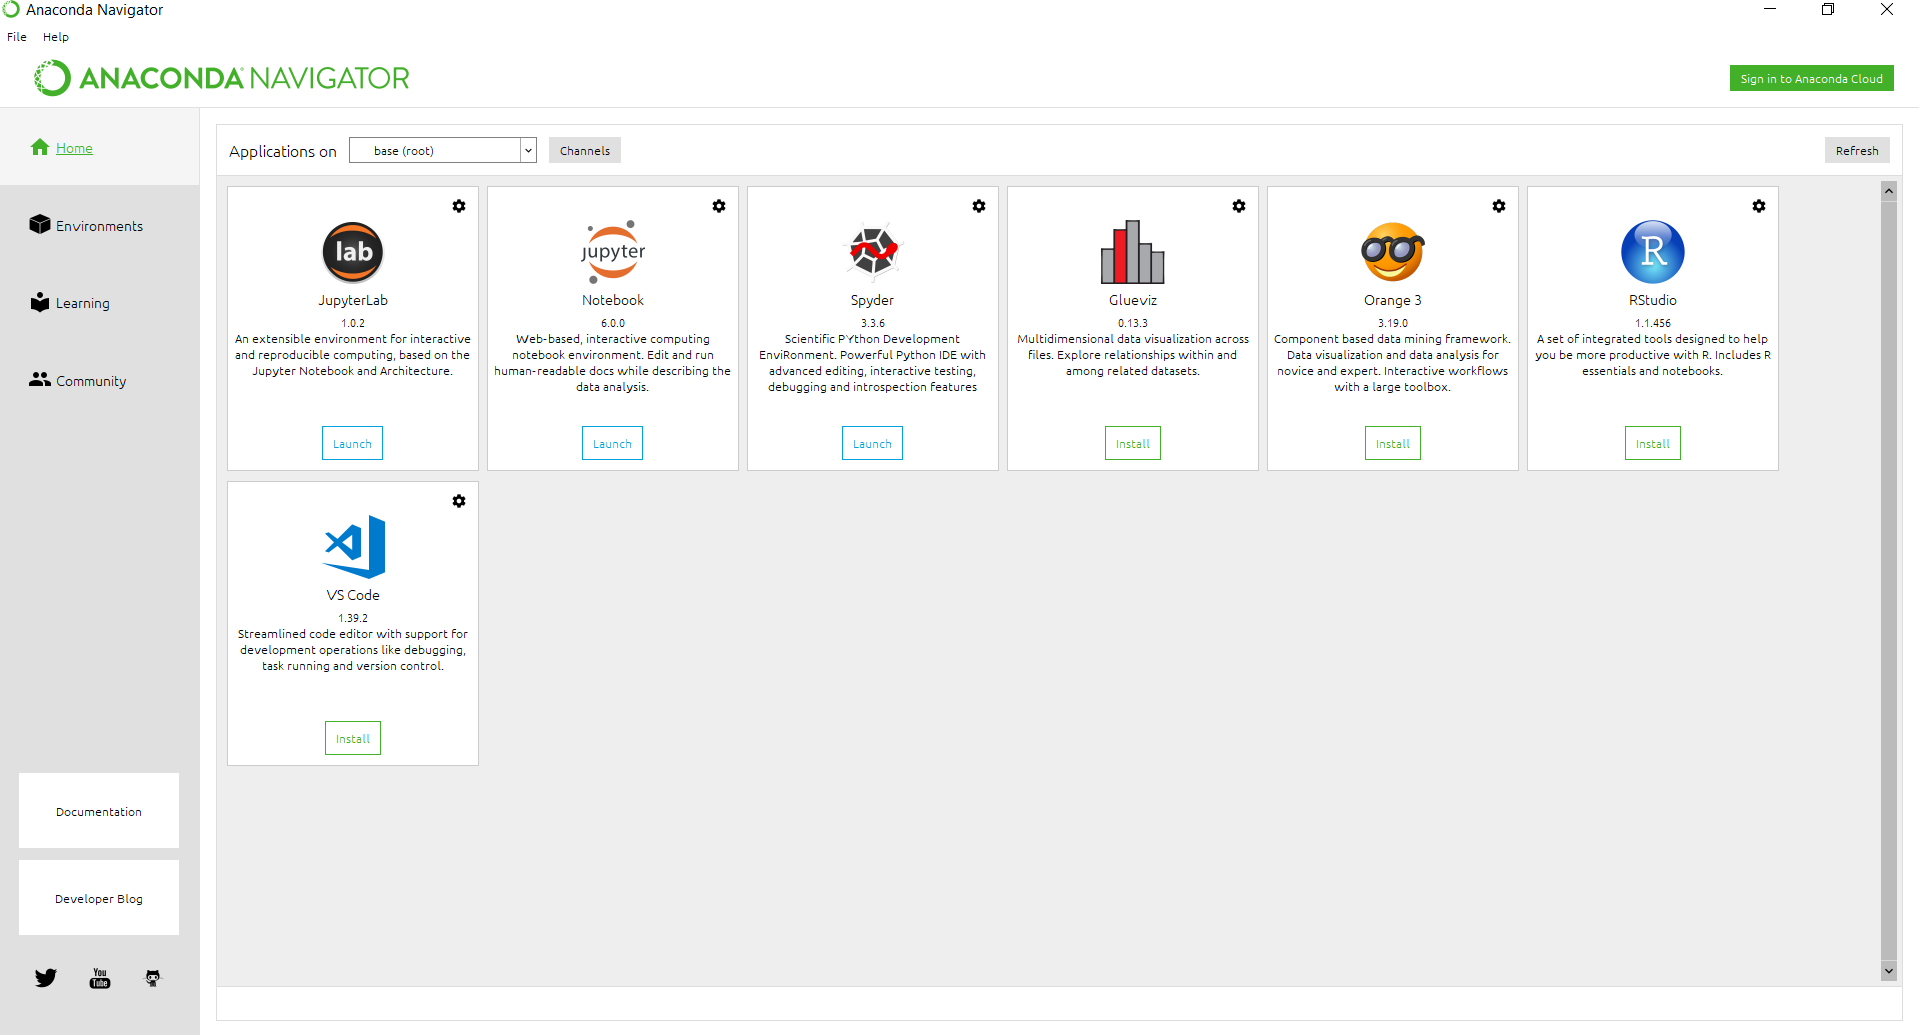
\includegraphics[scale=0.3]{figures/navigator}
    \caption{\textit{CLI in Command Prompt}}
    \label{Anaconda Navigator}
\end{figure}
\item ketikkan print("Hello World") dan run spyder
\begin{figure}[H]
    \centering
    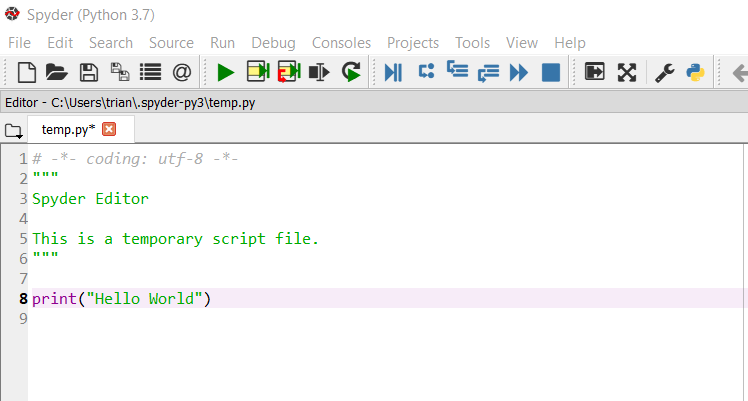
\includegraphics[scale=0.6]{figures/helloworld}
    \caption{\textit{Print Hello World}}
    \label{Print Hello World}
\end{figure}
\item hasilnya akan seperti ini
\begin{figure}[H]
    \centering
    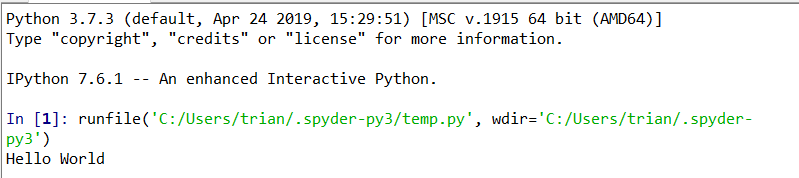
\includegraphics[scale=0.6]{figures/run}
    \caption{\textit{Hello World}}
    \label{Hello World}
\end{figure}
\end{enumerate}

\subsection{Automatic Login SIAP}
Buka Spyder lalu tuliskan script sebagai berikut.
\begin{verbatim}
from selenium import webdriver

print("Masukkan NPM Anda: ")
npm = input()
print("Masukkan Password Anda: ")
password = input()

options = webdriver.ChromeOptions()
driver = webdriver.Chrome(chrome_options=options)

driver.get("http://siap.poltekpos.ac.id/siap/besan.depan.php")

text = driver.find_element_by_name("user_name")
text.send_keys(npm)
paswd = driver.find_element_by_name("user_pass")
paswd.send_keys(password)

login = driver.find_element_by_name("login")
login.click()
\end{verbatim}
Kemudian save program dengan nama WA.py dan run program
\begin{figure}[H]
    \centering
    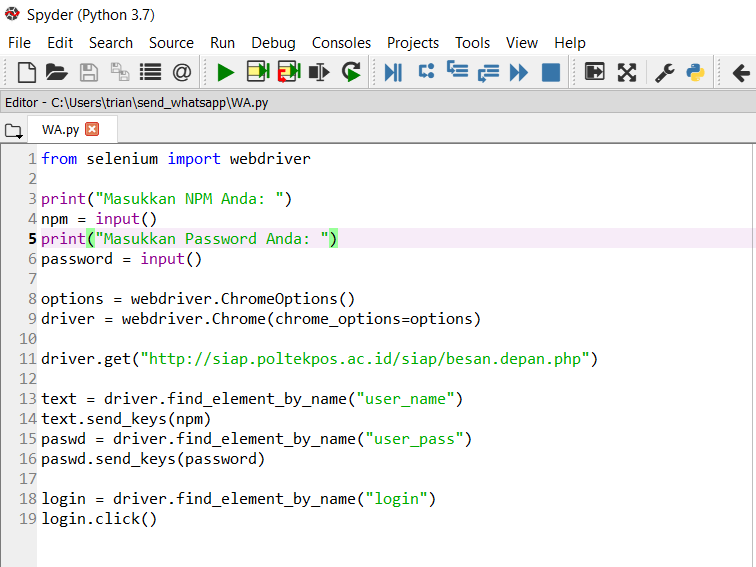
\includegraphics[scale=0.5]{figures/login}
    \caption{\textit{Automatic Login SIAP}}
    \label{Automatic1}
\end{figure}
Setelah di run maka akan diminta menginputkan NPM dan Password SIAP
\begin{figure}[H]
    \centering
    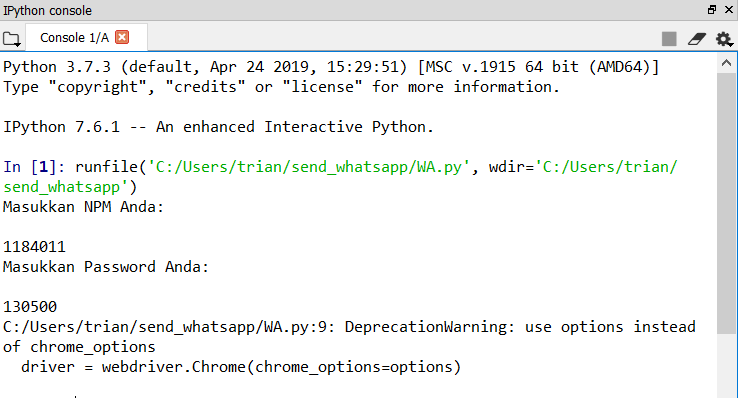
\includegraphics[scale=0.5]{figures/running}
    \caption{\textit{Hasil Running}}
    \label{Automatic2}
\end{figure}
Program selanjutnya akan membuka chrome secara otomatis dan mengetikkan NPM serta password yang telah diinputkan oleh user dan kemudian mengklik login.
\begin{figure}[H]
    \centering
    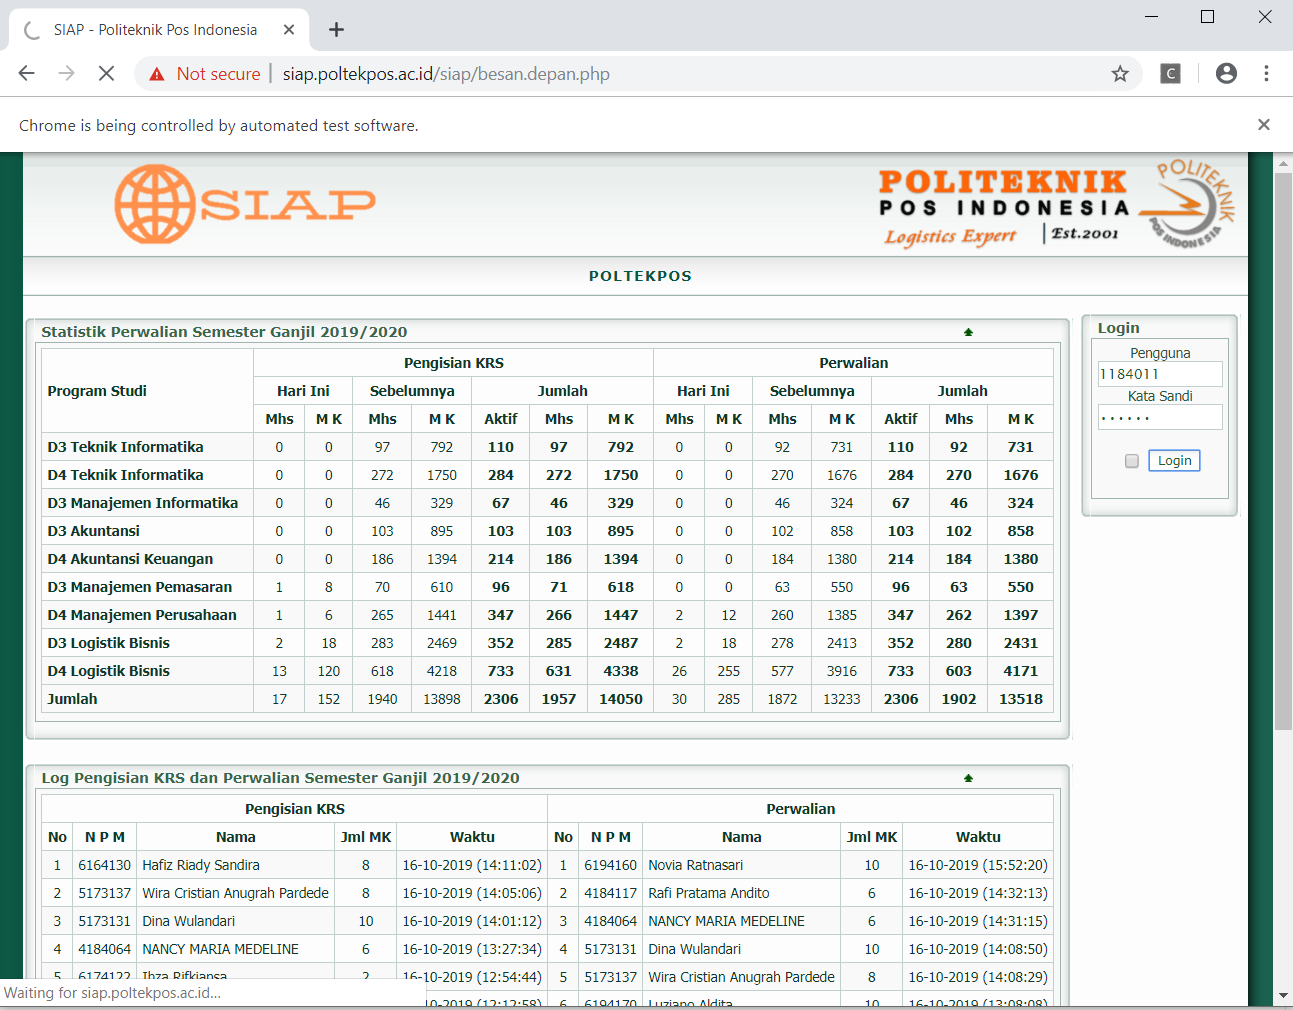
\includegraphics[scale=0.5]{figures/isi}
    \caption{\textit{Automatic Input dan Login}}
    \label{Automatic3}
\end{figure}
Login selesai
\begin{figure}[H]
    \centering
    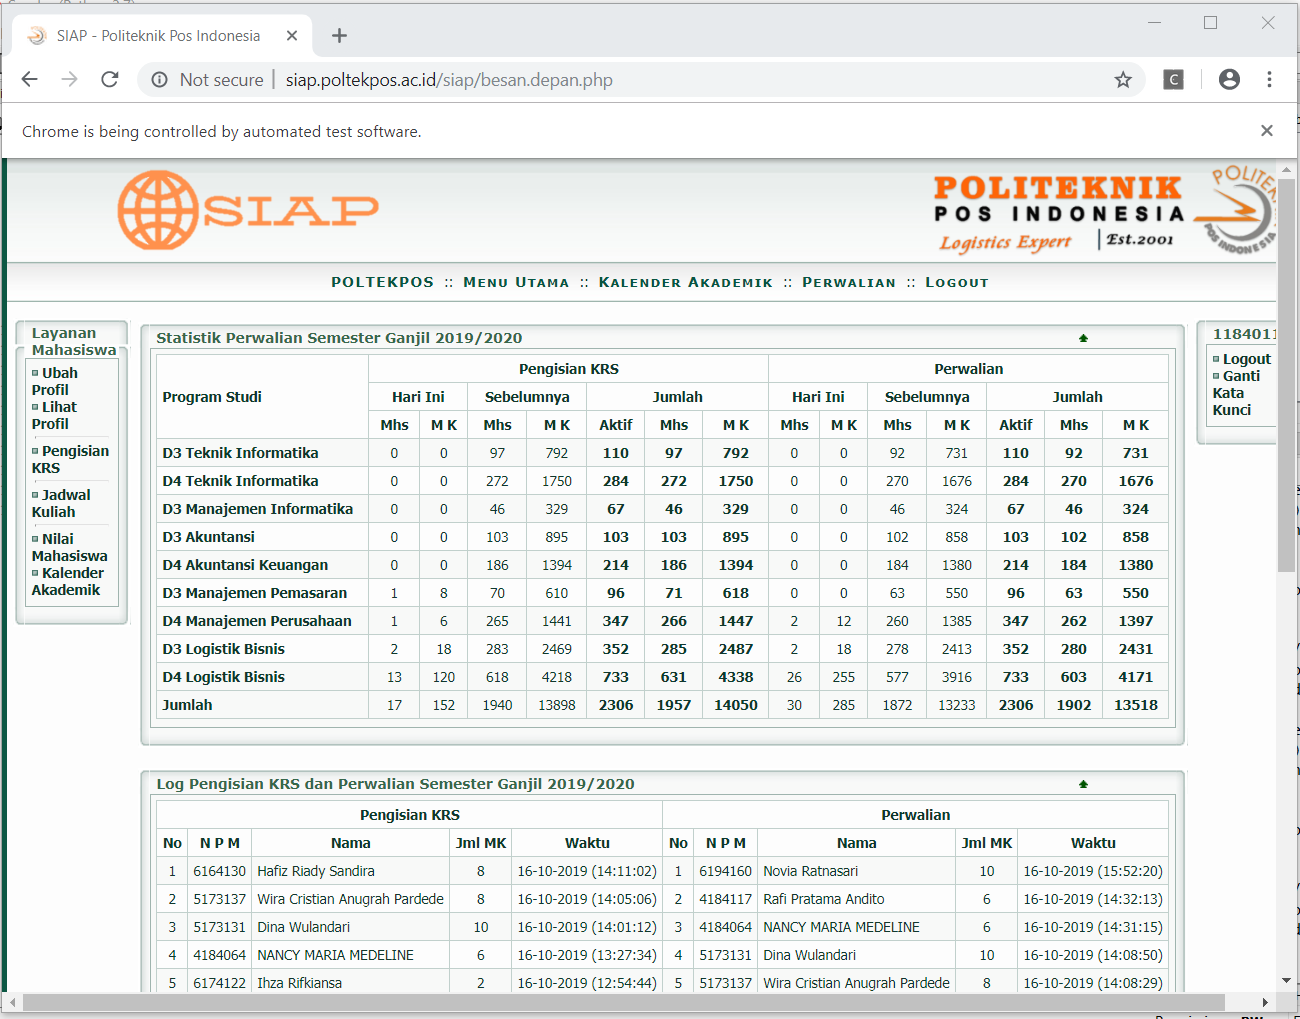
\includegraphics[scale=0.5]{figures/loginselesai}
    \caption{\textit{Automatic Input dan Login Selesai}}
    \label{Automatic4}
\end{figure}

\subsection{Pemakaian Variable Explorer}
Variable explorer akan secara otomatis terisi ketika kita membuat variable, pada variable explorer kita bisa melihat nama variable, tipe data, length, dan value dari variable tersebut.
\begin{figure}[H]
    \centering
    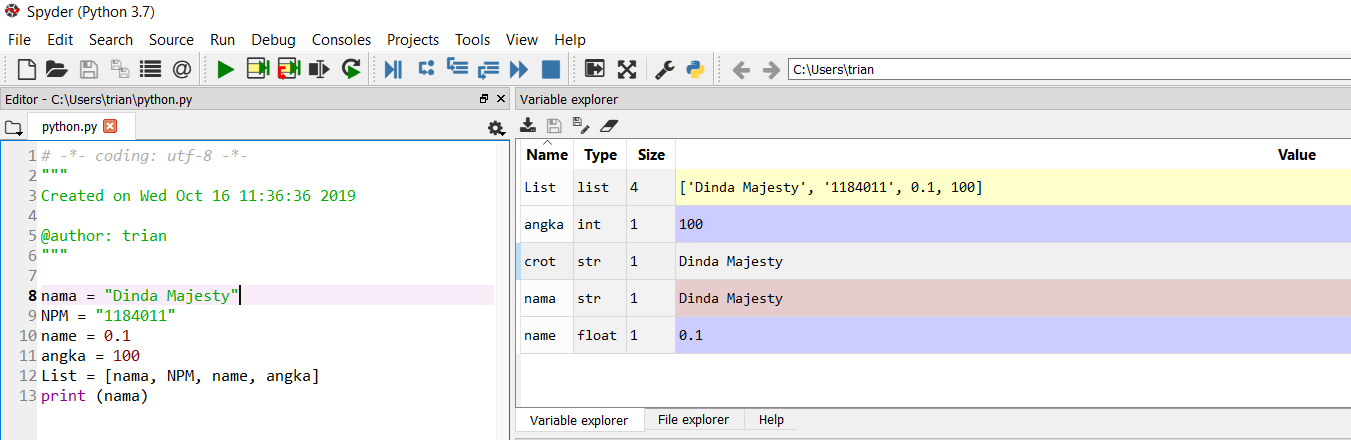
\includegraphics[scale=0.4]{figures/variable}
    \caption{\textit{Variable Explorer}}
    \label{Variable Explorer}
\end{figure}

\section{Indentasi}
\subsection{Penjelasan Indentasi}
Identasi adalah bagian paragraf yang menjorok ke dalam pada baris-baris paragraf. Mengatur indentasi dapat menggunakan tab atau spasi. Identasi digunakan oleh bahasa pemrograman python sebagai pengganti briket ({}) untuk membuka dan menutup fungsi. Error indentasi dapat terjadi apabila syntax tidak menggunakan tab atau space.
Contoh yang benar (menggunakan tab/spasi sebagai indentasi):
\begin{verbatim}
# blok percabangan if
if username == 'petanikode':
    print("Selamat Datang Admin")
    print("Silahkan ambil tempat duduk")

# blok percabangan for
for i in range(10):
    print i
\end{verbatim}
Contoh yang salah (tidak menggunakan tab/spasi):
\begin{verbatim}
# blok percabangan if
if username == 'petanikode':
print("Selamat Datang Admin")
print("Silahkan ambil tempat duduk")

# blok percabangan for
for i in range(10):
print i
\end{verbatim}

\subsection{Jenis-Jenis Error Indentasi}
IndentationError: unexpected indent. Error diatas terjadi apabila syntax kekurangan tab atau spasi.
\begin{figure}[H]
    \centering
    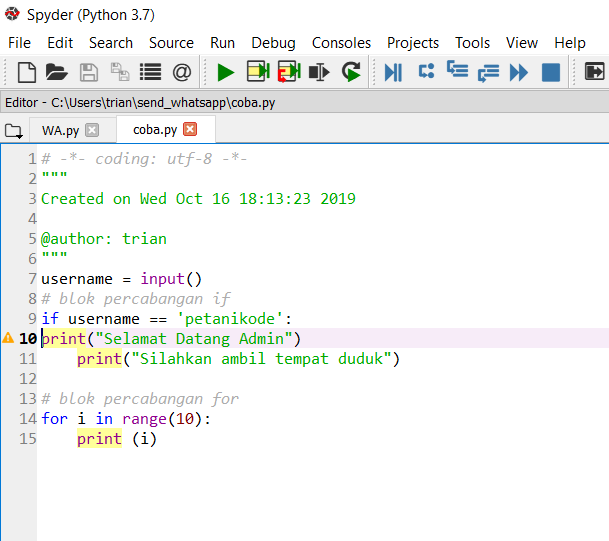
\includegraphics[scale=0.6]{figures/indentasi}
    \caption{\textit{Indentasi}}
    \label{Indentasi}
\end{figure}
Apabila di running akan memunculkan error sebagai berikut.
\begin{figure}[H]
    \centering
    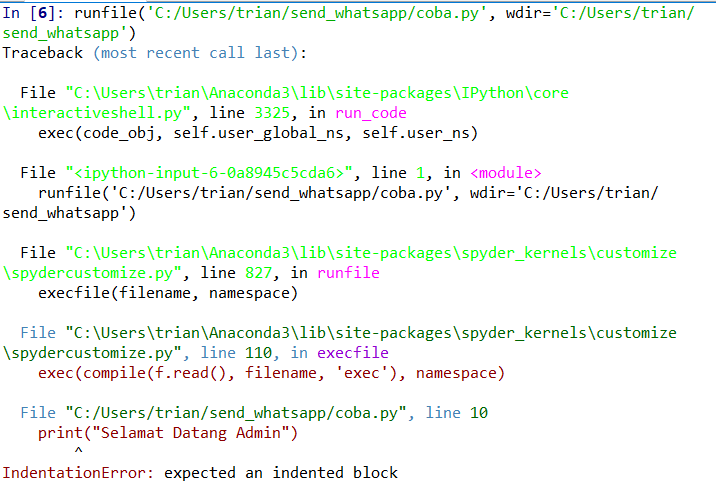
\includegraphics[scale=0.6]{figures/errorindentasi}
    \caption{\textit{Error Indentasi}}
    \label{Error Indentasi}
\end{figure}

\subsection{Cara Membaca Error}
Jika terjadi error maka cari di line berapa error terjadi, pada gambar berikut terdapat error indentasi pada line 10.
\begin{figure}[H]
    \centering
    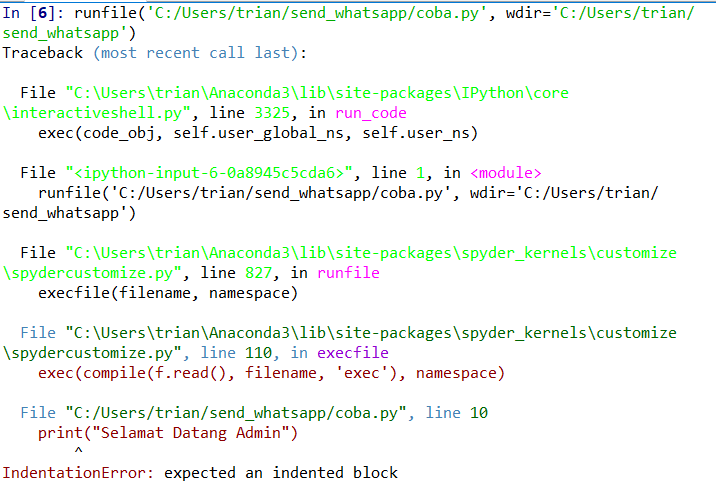
\includegraphics[scale=0.6]{figures/errorindentasi}
    \caption{\textit{Error}}
    \label{Error}
\end{figure}

\subsection{Cara Menangani Error}
Menangani error indentasi dapat dilakukan dengan cara menambahkan tab atau space pada line yang error.
Berikut syntax yang error.
\begin{figure}[H]
    \centering
    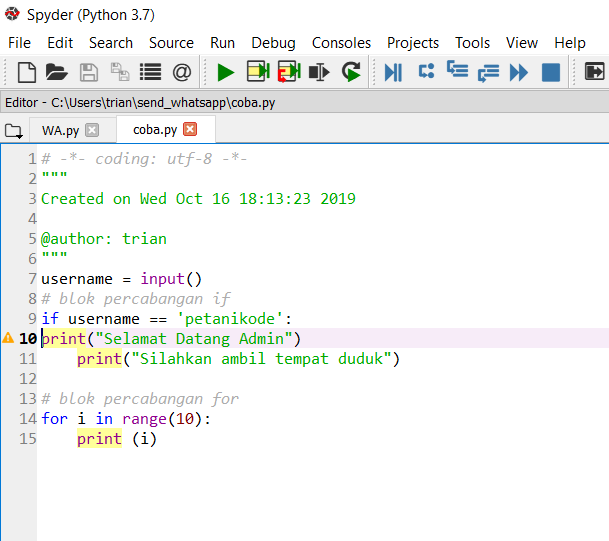
\includegraphics[scale=0.7]{figures/indentasi}
    \caption{\textit{Syntax Error}}
    \label{Syntax Error}
\end{figure}
Berikut syntax yang tidak error menggunakan tab/spasi (indentasi).
\begin{figure}[H]
    \centering
    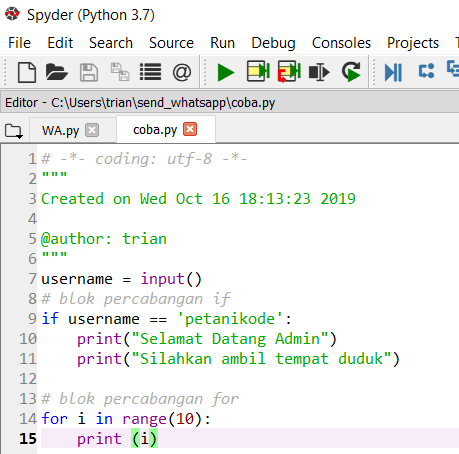
\includegraphics[scale=0.7]{figures/indentasicoy}
    \caption{\textit{Syntax yang Telah Diperbaiki}}
    \label{Syntax Error}
\end{figure}

\subsection{Link Youtube}
Berikut link youtube yang berisi jawaban dari pertanyaan-pertanyaan diatas.
\begin{verbatim}
https://www.youtube.com/channel/UCBadc75-CEWvCTTWkfUJEUg?view_as=subscriber
\end{verbatim}
